% N.B. one {latexonly} environment commented out so that its
% contents can be displayed in the HTML version of this template.
% Uncomment it for actual use!
%
% Use text editor to replace:
%
%       author   --- author's login name
%       thisdoc  --- document filename (as in thisdoc.tex, thisdoc.ps)
%       psiz     --- size of compressed PostScript file
%
%       Document_Date          --- current date
%       Document_Short_Title   --- header text for Postscript
%       Document_Long_Title    --- full document title
%       Author_Name            --- full author name
%       Author_City            --- Charlottesville, Socorro, etc.
%       Author_State           --- Virginia, New Mexico, etc.
%
%       (non-NRAO: also replace institute name/acronym and country?)
%

\documentclass{article}
\usepackage{html,makeidx,epsf}
\usepackage{graphicx}
\usepackage{amssymb}
\usepackage[overload]{empheq}

%\renewcommand{\bibname}{References}

%
% Add home page navigation button -- edit the URL!
%


\htmladdtonavigation{\htmladdnormallink
  {\htmladdimg{jetscalecropped.png}}{https://www.dropbox.com/s/jem3l3jabcyex9s/Curriculum_Vitae_Ilari_Angervuori.pdf?dl=0}}

%
% define hyperlink URLs:
%

\def\linkedin{https://www.linkedin.com/in/ilari-angervuori-0a1358160/}
\def\soundcloud{https://soundcloud.com/ilari-angervuori}
\def\github{https://github.com/Rugiero}
\def\pass{https://www.passwordstore.org/}
\def\cv{https://www.dropbox.com/s/jem3l3jabcyex9s/Curriculum_Vitae_Ilari_Angervuori.pdf?dl=0}
\makeindex

\begin{document}

%
%  Page formatting for Postscript output
%

\title{
{\bf A glimpse to my mind}
}

\author
{
Ilari Angervuori\\
}

\date
{
{Last update 11.02.2021}\\
}

\begin{center}
  \htmladdnormallink{Linkedin}{\linkedin}\\
  \htmladdnormallink{Soundcloud}{\soundcloud}\\
  \htmladdnormallink{GitHub}{\github} \\
  \htmladdnormallink{CV}{\cv}\\
\end{center}

%\begin{latexonly}
%\markright{Document_Short_Title}
\maketitle
% uncomment to run:
%\end{latexonly}

\tableofcontents

\pagebreak
\section{About me}
I am a mathematician and engineer from Finland. You can find about my professional achievements below.

I am keeping up a monthly blog what you can find in the blog posts section. It handles daily stuff encountered in my professional life. I hope you will find it interesting. 

In free time I love music, literature, long walks, coffee and beer.


\begin{figure}
  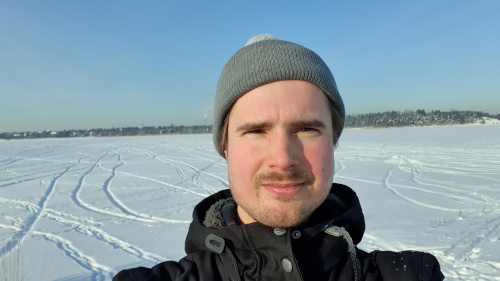
\includegraphics[width=\linewidth]{me1.jpg}
  \caption{Me in my beloved home town Helsinki in the middle of summer (well, technically in Espoo, Otaniemi)}
\end{figure}

\subsection{Education}
\begin{itemize}
\item 2016 Bachelor of Science University of Helsinki\\
\item 2018 Master of Philosophy University of Helsinki
\end{itemize}
\subsection{Research}

\begin{itemize}
\item Downlink Coverage and Rate Analysis of Low Earth Orbit Satellite Constellations Using Stochastic Geometry
  Okati, N., Riihonen, T., Korpi, D., Angervuori, I. Wichman, R., Aug 2020, In : IEEE Transactions on Communications. 68, 8, p. 5120-5134 9079921.\\
\item A. Yastrebova et al., "Theoretical and Simulation-based Analysis of Terrestrial Interference to LEO Satellite Uplinks," GLOBECOM 2020 - 2020 IEEE Global Communications Conference, Taipei, Taiwan, 2020, pp. 1-6, doi: 10.1109/GLOBECOM42002.2020.9347980.
\end{itemize}


\section{Blog posts 2021}
General thoughts on mathematics and engineering, practical instructions and artistic non sense. The themes of this blog are much inspired by challenges encountered in my professional life.

\subsection{January}
\subsubsection{Poisson process on a sphere}
Of course, Poisson process can be generalized to an arbitrary manifold. Particularly Poisson point process on a sphere is useful. Nicely enough, Poisson process on a sphere is equivalent to process in a two dimensional area $ A = [-\pi,\pi] \times [-1,1]$ through the area preserving mapping from $A$ to surface of a sphere
\begin{equation}
  (x,y) \mapsto (r,x,\sin(y)) \nonumber.
\end{equation}


Resulting process interpreted in geographical coordinates $(r,\theta,\varphi)$ is a Poisson point process on a sphere of radius $r$.  Following codes returns a scatter plot of Poisson points on the unit sphere.



GNU/Octave or Matlab:
\begin{verbatim}
%Plot random points on a unit sphere. Returns the points in a vector ref in cartesian coordinates
function refc = poissononsphere(density)
  yMin = -1; yMax = 1;
  xMin=-pi; xMax = pi;
  
  xDelta=xMax-xMin;yDelta=yMax-yMin; %Rectangle dimensions
  numbPoints=poissrnd(density);    %Number of points in the area is a Poisson variable of intensity given as density
  x=xDelta*(rand(numbPoints,1))+xMin;    %Pick points from uniform distribution
  y=yDelta*(rand(numbPoints,1))+yMin;    %Map referencepoints to geographical coordinates
  ref = [x y]';

  refs = [x'; asin(y)'];%Map geographical coordinates to Cartesian coordinates on a unit circle
  r = 1;
  refc = [r*sin(refs(2,:)+pi/2).*cos(refs(1,:)+pi);...
          r*sin(refs(2,:)+pi/2).*sin(refs(1,:)+pi);...
          r*cos(refs(2,:)+pi/2)];

  figure(1)    %Plot
  [X, Y, Z] = sphere;
  surf(X,Y,Z,'EdgeColor','none','FaceColor','black');
  hold on
  scatter3(refc(1,:),refc(2,:),refc(3,:),10,...
           'MarkerFaceColor','yellow',...
           'MarkerEdgeColor','red');
  axis equal
end
\end{verbatim}

Python:

\begin{verbatim}
import numpy as np
import scipy.stats
import matplotlib.pyplot as plt
from mpl_toolkits.mplot3d import axes3d

#Rectangle dimension
xMin=-np.pi;xMax=np.pi;
yMin=-1;yMax=1;
xDelta=xMax-xMin;yDelta=yMax-yMin; #rectangle dimensions

#Density parameter of the Poisson point process. Mean number of points on the sphere
lambda0=1000; 

#Simulate Poisson point process

#Number of point in the area is a Poisson variable of intensity lambda0
numbPoints = scipy.stats.poisson( lambda0 ).rvs()
x = xDelta*scipy.stats.uniform.rvs(0,1,((numbPoints,1)))+xMin
y = yDelta*scipy.stats.uniform.rvs(0,1,((numbPoints,1)))+yMin

#Transform to geographical coordinates
x = x
y = np.arcsin(y)
#Plotting
fig = plt.figure()
ax = plt.axes(projection="3d")
ax.scatter(np.sin(y+np.pi/2)*np.cos(x+np.pi),np.sin(y+np.pi/2)*np.sin(x+np.pi),np.cos(y+np.pi/2), color='r' )
plt.show()
  
\end{verbatim}

Wolfram Language:
\begin{verbatim}
(*lambda is the mean number of points on the unit sphere*) 
  poissononsphere[lambda_] := 
  Module[{nrofpoints, phi, theta, radius, refc, polarp}, 
   nrofpoints = RandomVariate[PoissonDistribution[lambda]];
   polarp = 
    Table[{RandomVariate[UniformDistribution[{-Pi, Pi}]], 
      ArcSin[RandomVariate[UniformDistribution[{-1, 1}]]]}, 
     nrofpoints];
   radius = 1;
   refc = 
    Table[{radius*Sin[polarp[[i]][[2]] + Pi/2]*
       Cos[polarp[[i]][[1]] + Pi],
      radius*Sin[polarp[[i]][[2]] + Pi/2]*Sin[polarp[[i]][[1]] + Pi],
      radius*Cos[polarp[[i]][[2]] + Pi/2]}, {i, nrofpoints}];
   refc
   ];
   ListPointPlot3D[poissononsphere[500], BoxRatios -> {1, 1, 1}]  
\end{verbatim}

\begin{figure}
  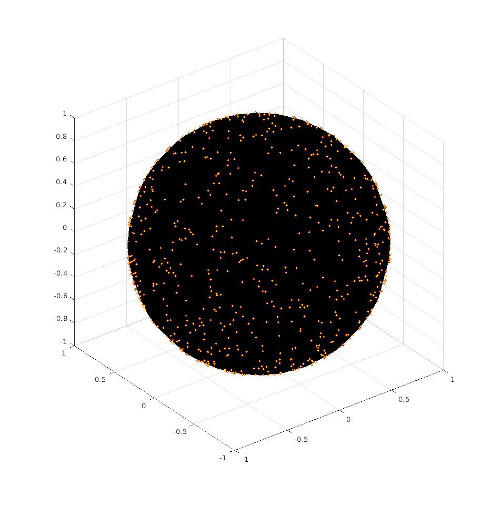
\includegraphics[width=\linewidth]{poissononsphere.jpg}
  \caption{Are the stars Poisson distributed in the sky?}
\end{figure}

\begin{figure}
  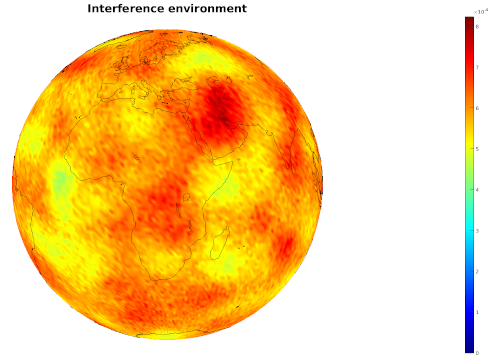
\includegraphics[width=\linewidth]{interferenceenvironment.png}
  \caption{Poisson distributed transmitters and the aggregate signal strength in a satellite by location. Poisson assumption is reasonable in many situations, but, well, here the sea areas are a bit overrepresented.  }
\end{figure}

References:
\bibitem{theoryofpoint} D. J. Daley and D. Vere-Jones, ``The General Poisson Process'' in {\em An introduction to the theory of point processes.} New York: Springer, 2003, pp. 39. 
\bibitem{2} Stoyan, Dietrich. et al. \em{Stochastic Geometry and Its Applications}. 3rd ed. Chichester: Wiley, 2013. Print.




\subsection{February}
\subsubsection{Controlling your passwords with pass}
Pass is a nice unix style free and open source wallet for keeping your passwords safe. Here is a brief look how to set it up in Ubuntu.

\begin{itemize}
\item Install the application in the terminal \\
\begin{verbatim}
sudo apt install pass  
\end{verbatim}
\item Check for existing GPG keys \\
\begin{verbatim}
gpg --list-keys 
\end{verbatim}
\item If no keys were found generate a key pair \\
\begin{verbatim}
gpg --generate-key
\end{verbatim}
\item Copy the name of the key and initalize pass\\
\begin{verbatim}
pass init ABCDEFGHIJKLMNOPQRSTUV1234, 
\end{verbatim}
where ABCDEFGHIJKLMNOPQRSTUV1234 is the name of the key.
\item Generate a password with \\
\begin{verbatim}
pass generate keyfolder/newkey 
\end{verbatim}
List passwords
\begin{verbatim}
pass
\end{verbatim}
Copy a password to clipboard \\
\begin{verbatim}
pass keyfolder/newkey -c
\end{verbatim}
For more commands
\begin{verbatim}
man pass
\end{verbatim}
\end{itemize}

Connect pass to git so it is easy to keep track of changes with multiple machines.

\begin{itemize}
\item Export your public and private key to a file with \\
  \begin{verbatim}
gpg --export --output public.key ABCDEFGHIJKLMNOPQRSTUV1234 
gpg --export-secret-key --output private.key ABCDEFGHIJKLMNOPQRSTUV1234,
  \end{verbatim}
  where ABCDEFGHIJKLMNOPQRSTUV1234 is your key name.\\
\item Now we can initilize the git reporisoritory with these keys. Move public.key and private.key through a safe channel to a computer you wish to use pass in. Import the keys to the machine \\
\begin{verbatim}
gpg --import public.key
gpg --import private.key
\end{verbatim}
\item After importing keys to a new machine you can initilize pass
\begin{verbatim}
pass init ABCDEFGHIJKLMNOPQRSTUV1234
\end{verbatim}

\item Initalize your git repository. Make a new repository named pass-store e.g. to GitHub if you are doing this first time before the following commands\\
\begin{verbatim}
pass git init 
pass git remote add origin git@repo.com:myname/pass-store
 \end{verbatim}
\item Get password data from the server (from a non-empty repository, otherwise skip)
\begin{verbatim}
pass git pull origin master --allow-unrelated-histories
\end{verbatim}
\item Do some changes and pass will automatically commit them. Push and set upstream \\
\begin{verbatim}
pass git push --set-upstream origin master 
\end{verbatim}
\item From here on you can use the familiar git commands \\
\begin{verbatim}
pass git pull 
pass git push 
\end{verbatim}
\end{itemize}
Stay safe :)


References:

 \bibitem[1]{pass}\htmladdnormallink{Password Store}{\pass}

\end{document}
%
% optional post-title formatting for PostScript
%
\parindent0pt
\parskip2.5ex plus 0.5ex minus 0.5ex

